\documentclass{beamer}

\usepackage[utf8]{inputenc}
\usepackage{amsmath}
\usepackage{graphicx}
\usepackage{xcolor}

\title{Elevator Controller}
\author{Antoine Karam, Ghady Youssef}
\institute{Saint Joseph University of Beirut}
\date{January 10, 2025}

\begin{document}

\frame{\titlepage}

\section{Introduction}
\begin{frame}
    \frametitle{Introduction}
    \begin{itemize}
        \item Overview of the project
        \item Objectives and goals
        \item Design considerations
    \end{itemize}
\end{frame}

\section{Firmware Architecture}
\begin{frame}
    \frametitle{Firmware Architecture}
    \begin{figure}[h]
        \centering
        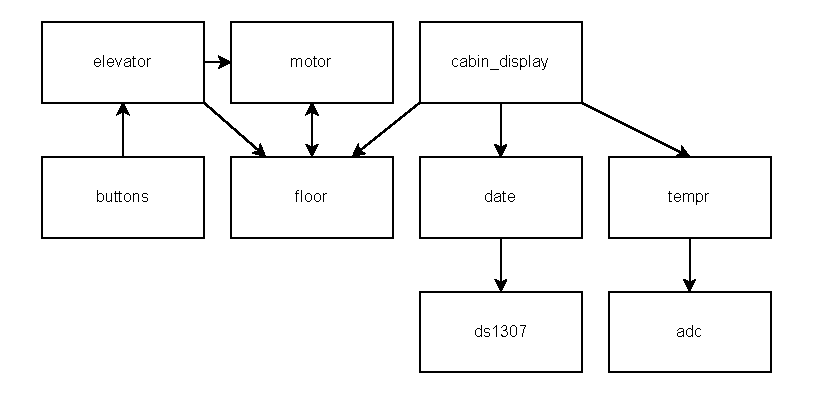
\includegraphics[width=\textwidth]{assets/block-diagram.pdf}
    \end{figure}
\end{frame}

\section{Drivers}
\begin{frame}
    \frametitle{Drivers}
    \begin{itemize}
        \item \textbf{Temperature: LM35}
              \begin{itemize}
                  \item Measures temperature
                  \item Connected to ADC
                  \item Two functions for temperature retrieval
              \end{itemize}
        \item \textbf{Real-Time Clock: DS1307}
              \begin{itemize}
                  \item Retrieves time and date
                  \item Utilizes I$^2$C communication
                  \item API provides functions to access date and time
              \end{itemize}
    \end{itemize}
\end{frame}

\section{Display}
\begin{frame}
    \frametitle{Display}
    \begin{itemize}
        \item \textbf{Floor Display}
              \begin{itemize}
                  \item Shows current floor
                  \item Monitors the switches on each stop to update global state
              \end{itemize}
        \item \textbf{Cabin Display}
              \begin{itemize}
                  \item Displays time, date, and temperature
                  \item Cycles every 10 seconds
              \end{itemize}
    \end{itemize}
\end{frame}

\section{Motor}
\begin{frame}
    \frametitle{Motor}
    \begin{itemize}
        \item Moving the cabin between floors
        \item Critical for scheduler and floor display
        \item Prevent abrupt direction changes
    \end{itemize}
\end{frame}

\section{Scheduler}
\begin{frame}
    \frametitle{Scheduler}
    \begin{itemize}
        \item Determine next floor for the elevator
        \item Avoid abrupt direction changes for safety
        \item Efficient handling of floor requests
        \item Queue management: Separate queues for up/down requests
    \end{itemize}
\end{frame}

\begin{frame}
    \frametitle{Scheduler}
    \begin{figure}[h]
        \centering
        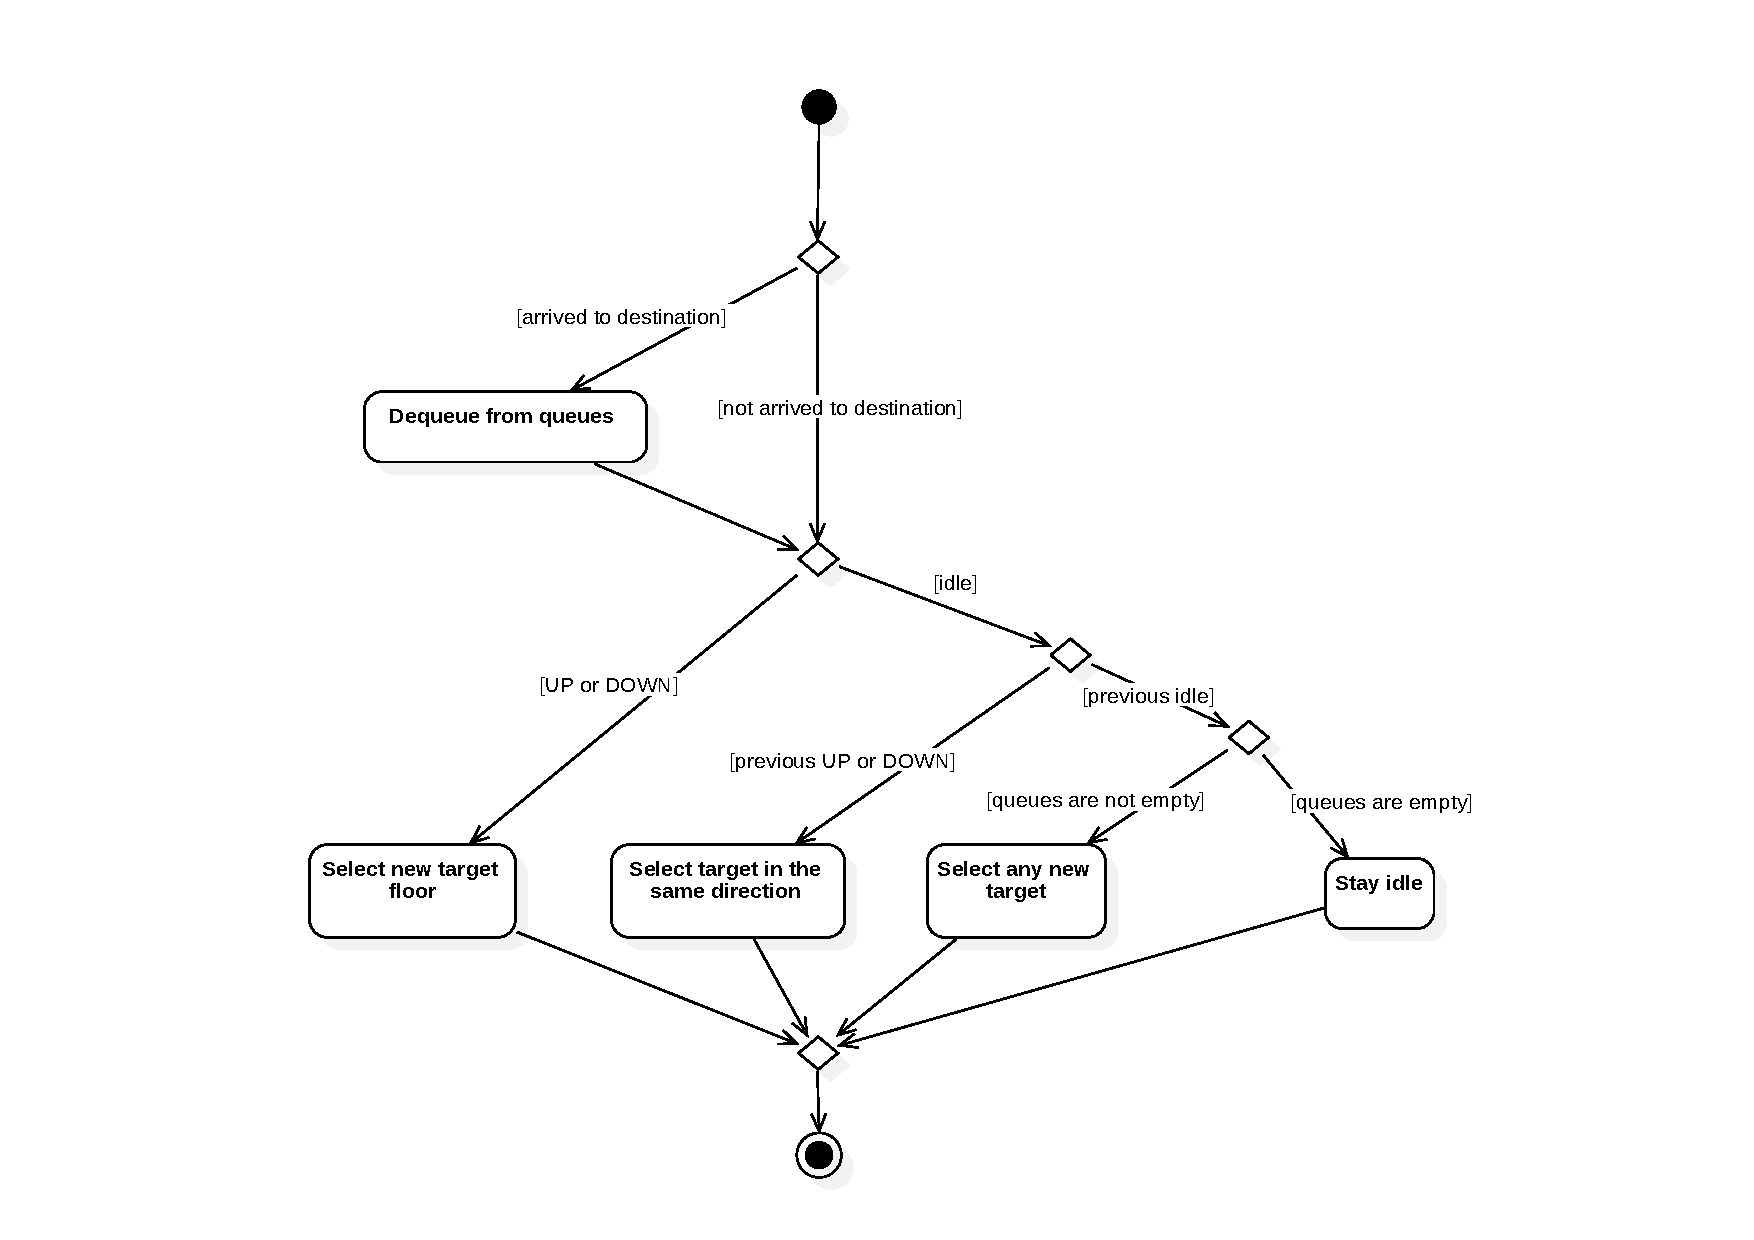
\includegraphics[width=\textwidth]{assets/scheduler.pdf}
    \end{figure}
\end{frame}

\section{Development Workflow}
\begin{frame}
    \frametitle{Development Workflow}
    \begin{itemize}
        \item \textbf{Version Control}
              \begin{itemize}
                  \item Git and GitHub for collaboration
                  \item Task management using GitHub Issues
                  \item Branching strategy for feature development
              \end{itemize}
        \item \textbf{Continuous Integration}
              \begin{itemize}
                  \item \texttt{clang-format} and \texttt{cppcheck} for code quality
                  \item GitHub Actions for CI pipelines
                  \item Live documentation available
              \end{itemize}
    \end{itemize}
\end{frame}

\section{Documentation}
\begin{frame}
    \frametitle{Documentation with \texttt{doxygen}}
    \begin{figure}[h]
        \centering
        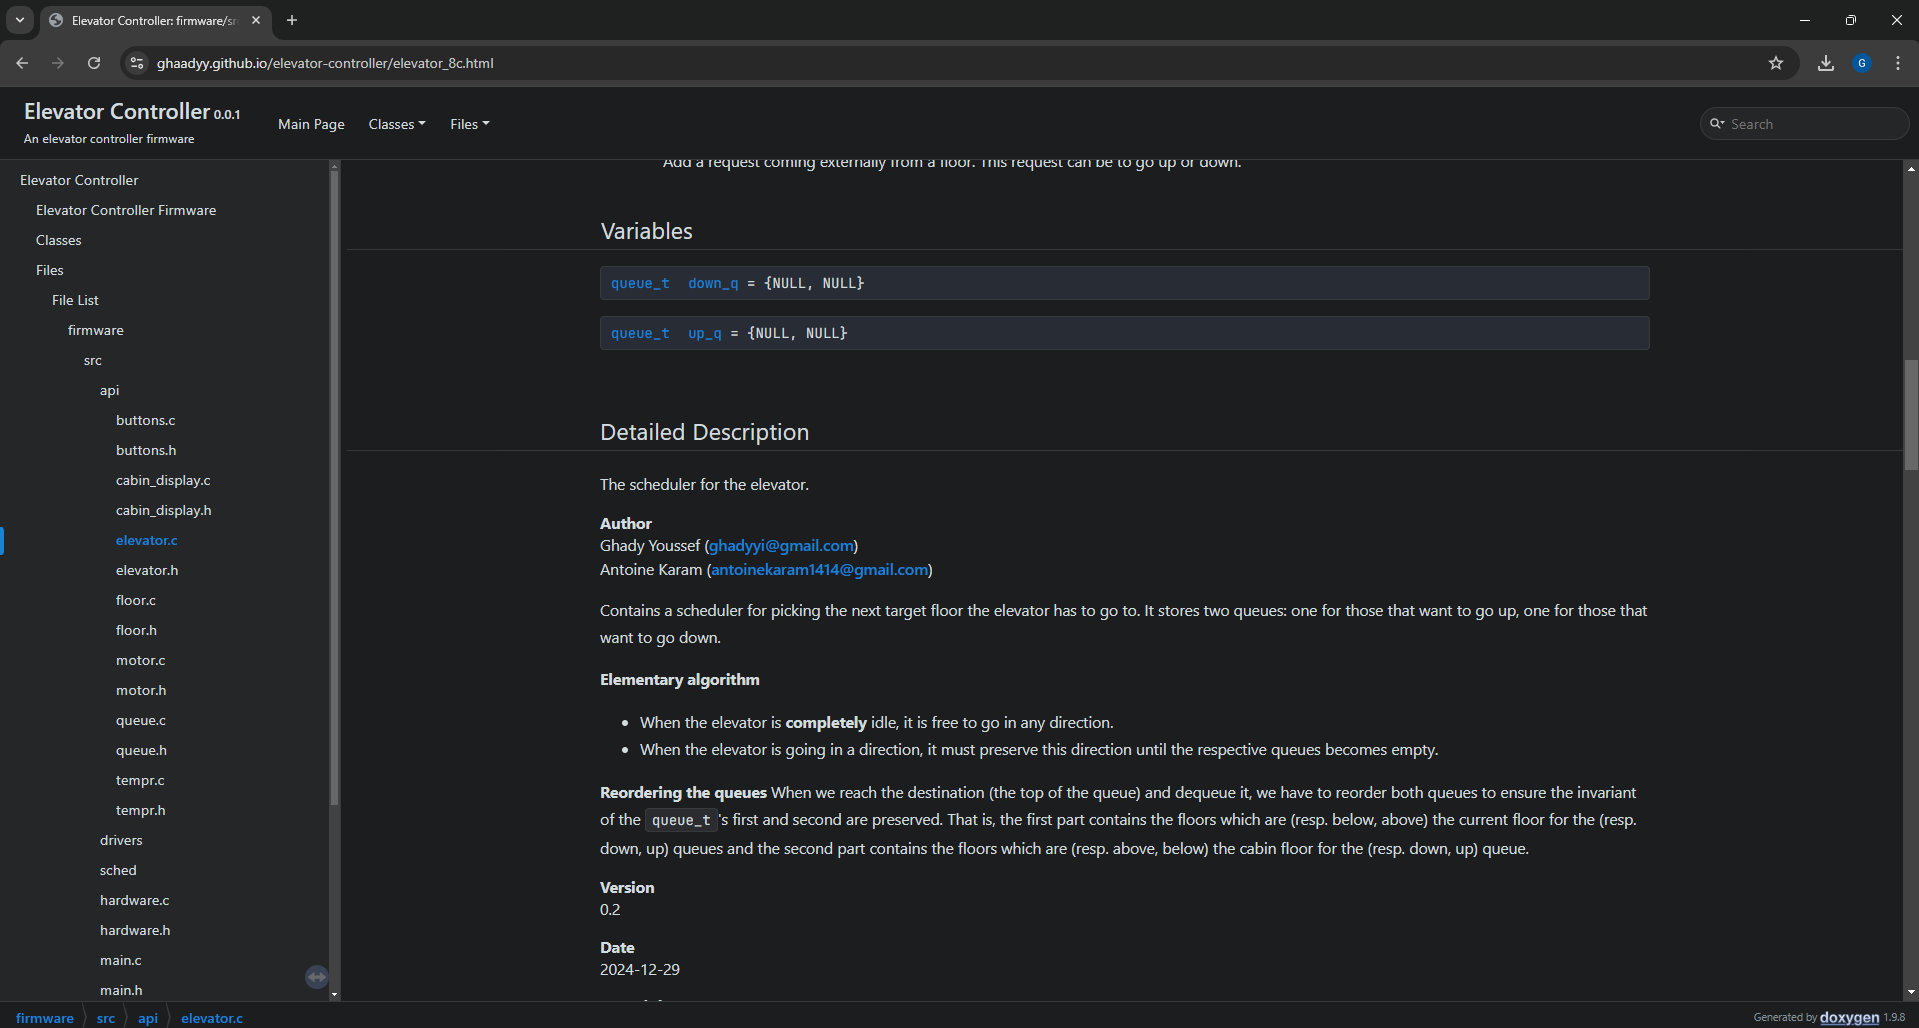
\includegraphics[width=1\textwidth]{assets/docs.png}
        \caption{
            Available at \href{https://ghaadyy.github.io/elevator-controller/}{https://ghaadyy.github.io/elevator-controller/}
        }
    \end{figure}
\end{frame}

\section{Challenges}
\begin{frame}
    \frametitle{Challenges}
    \begin{itemize}
        \item Designing efficient elevator scheduling algorithm
        \item Debugging logical errors
    \end{itemize}
\end{frame}

\section{Future Work}
\begin{frame}
    \frametitle{Future Work}
    \begin{itemize}
        \item Error detection and handling for power failures and motor issues
    \end{itemize}
\end{frame}

\end{document}
